%\documentclass[14pt,a4paper]{article}
\documentclass{article}

\usepackage[utf8]{inputenc}
\usepackage[french]{babel}
\usepackage{amsmath}
\usepackage{amssymb}
\usepackage{amsfonts} 
\usepackage{enumitem}
\usepackage{graphicx}
\usepackage{stmaryrd}
\usepackage{mathtools}
\usepackage{listings}
\usepackage{fullpage}
\usepackage{color}
\usepackage[table]{xcolor}
\usepackage{listings}
\usepackage{pdfpages}
\usepackage{titling}
\usepackage{titlesec}
\usepackage{hyperref}
\usepackage{tikz}
\usepackage{graphicx}
\usepackage{subcaption}
\usepackage[left=3cm,right=3cm,top=3cm,bottom=3cm]{geometry}
\usepackage{wrapfig}
\usepackage{tikz}
\newcommand*\circled[1]{\tikz[baseline=(char.base)]{
            \node[shape=circle,draw,inner sep=2pt] (char) {#1};}}
\newcommand{\subsubsubsection}[1]{\paragraph{#1}\mbox{}\\}
\renewcommand{\thesection}{\arabic{section}}
\setlength{\footskip}{15pt}
\definecolor{darkWhite}{rgb}{0.94,0.94,0.94}
\lstset{
aboveskip=3mm,
belowskip=-2mm,
backgroundcolor=\color{darkWhite},
basicstyle=\footnotesize,
breakatwhitespace=false,
breaklines=true,
captionpos=b,
commentstyle=\color{red},
deletekeywords={...},
escapeinside={\%*}{*)},
extendedchars=true,
framexleftmargin=16pt,
framextopmargin=3pt,
framexbottommargin=6pt,
frame=tb,
keepspaces=true,
keywordstyle=\color{blue},
language=C,
literate=
{²}{{\textsuperscript{2}}}1
{⁴}{{\textsuperscript{4}}}1
{⁶}{{\textsuperscript{6}}}1
{⁸}{{\textsuperscript{8}}}1
{€}{{\euro{}}}1
{é}{{\'e}}1
{è}{{\`{e}}}1
{ê}{{\^{e}}}1
{ë}{{\¨{e}}}1
{É}{{\'{E}}}1
{Ê}{{\^{E}}}1
{û}{{\^{u}}}1
{ù}{{\`{u}}}1
{â}{{\^{a}}}1
{à}{{\`{a}}}1
{á}{{\'{a}}}1
{ã}{{\~{a}}}1
{Á}{{\'{A}}}1
{Â}{{\^{A}}}1
{Ã}{{\~{A}}}1
{ç}{{\c{c}}}1
{Ç}{{\c{C}}}1
{õ}{{\~{o}}}1
{ó}{{\'{o}}}1
{ô}{{\^{o}}}1
{Õ}{{\~{O}}}1
{Ó}{{\'{O}}}1
{Ô}{{\^{O}}}1
{î}{{\^{i}}}1
{Î}{{\^{I}}}1
{í}{{\'{i}}}1
{Í}{{\~{Í}}}1,
morekeywords={*,...},
numbers=left,
numbersep=10pt,
numberstyle=\tiny\color{black},
rulecolor=\color{black},
showspaces=false,
showstringspaces=false,
showtabs=false,
stepnumber=1,
stringstyle=\color{gray},
tabsize=4,
title=\lstname,
}



\title{\textbf{Projet de groupe : {\bfseries Outil interactif de Visualisation et Manipulation de Séries Temporelles Biologiques }- "ViMaSTBio"}}



\author{
  \\%
  \\
  Lucas \textsc{Deswarte}, Dorian \textsc{Malguid}, David \textsc{Malvoisin}, \\
  Mathilde \textsc{Puche}, Oscar \textsc{Saadate}}

\date{25 mars 2019}

\begin{document}

\vbox{\vspace{-1cm}

    \centering
    
\includegraphics[scale = .35]{images/LogoECN.png}
    \vspace{1.5cm}
    \maketitle
  }
  
\thispagestyle{empty}
  
\vfill
\begin{flushright} 
      Encadrants du projet : Olivier \textsc{Roux} et Samuel \textsc{Buchet}
\end{flushright} 

  
\renewcommand{\contentsname}{Sommaire}

\noindent

\clearpage
\begingroup
\let\cleardoublepage\clearpage
\setcounter{page}{1}
\tableofcontents
\endgroup
\newpage
\section{Introduction}
\bigbreak
\bigbreak

Ce projet de groupe a pour but de nous faire travailler à plusieurs sur des notions vues en cours afin de les approfondir et les appliquer à un cas concret. Il a  été réalisé en groupe de cinq composé de deux étudiants en SI et trois en GI, ce qui a permis une polyvalence des connaissances. 
\newline 

M. Samuel Buchet et M. Olivier Roux travaillent actuellement sur une analyse de données de régulations biologiques. Pour ce faire, ils ont utilisé jusqu'à présent des représentations faites sur papier, rendant le travail fastidieux et difficile à exploiter du fait du nombre considérable de données et de leur évolution rapide. C'est dans ce contexte qu'ils nous ont demandé de créer un outil interactif permettant la manipulation et la visualisation des données biologiques qu'ils étudient. 


\bigbreak
\bigbreak
\bigbreak

\section{Présentation du projet}
\bigbreak
\bigbreak

\subsection{Contexte}
Pour analyser les données biologiques et comprendre les mécanismes qui régissent le passage d'un gène d'un état à un autre, il est nécessaire de prendre en compte plusieurs paramètres. 
\newline 

Premièrement, les échantillons d'étude pouvant aller jusqu'à regrouper plusieurs milliers de gènes, il faut sélectionner ceux qui sont pertinents pour effectuer une analyse précise. De même, une fenêtre temporelle d'étude doit être définie afin d'étudier les instants contenant les données exploitables.
\newline 

Une fois les gènes et la fenêtre de temps sélectionnés, il est intéressant pour les biologistes de pouvoir visualiser, dans une même représentation graphique, l'évolution temporelle de tous ces gènes.
\newline 

De plus, il leur faut pouvoir observer, à un instant donné, l'état de tous les gènes sélectionnés. Cela permet de trouver des correlations entre la transition d'un gène d'un état à un autre et l'état courant de chacun des autres gènes. M. Samuel Buchet et M. Olivier Roux ont choisi de représenter les gènes par des automates et ont déjà trouvé des conditions sur les transitions.
\newline 

Afin de vérifier ces dernières, une représentation graphique de l'évolution supposée par les automates et leurs transitions peut permettre aux biologistes d'effectuer une comparaison rapide avec la première courbe réelle.
\newline 

Ainsi, l'analyse des mécanismes biologiques requiert plusieurs étapes de manipulation et de représentation de données qui peuvent s'avérer être très fastidieuses et chronophages si elles sont effectuées à la main. 
\bigbreak
\bigbreak
\subsection{Objectifs}
Notre objectif a alors été de créer un outil facilitant la mise en oeuvre des étapes précédemment décrites. Cet outil devait afficher les représentations dynamiques suivantes :
\begin{itemize}[leftmargin=1.5cm]
    \item[•] Représentation temporelle des données fournies sur l'évolution des gènes, sous forme de chronogramme. Nous l'appellerons "\textit{chronogramme réel}" par la suite ;
    \item[•] Représentation des automates étant liés aux états des gènes à un instant donné. Les différents états activés devaient être mis en évidence par une couleur ; 
    \item[•] Représentation de l'évolution des gènes supposée par les automates sous forme de chronogramme discrétisé. Nous l'appellerons "\textit{chronogramme estimé}" par la suite.
\end{itemize}
\bigbreak
\noindent De plus, l'outil devait assurer les fonctionnalités suivantes :

\begin{itemize}[leftmargin=1.5cm]


\item[•]\textbf{sélection des gènes} retenus pour l'étude, par la selection d'un fichier donné  ;

\item[•]\textbf{sélection d'un gène} en particulier sur le chronogramme réel. Les seuils du gène ainsi isolé seront alors affichés et pourront être modifiés à l'aide d'un curseur déplaçable ;

\item[•]\textbf{sélection d'une fenêtre temporelle} pour l'étude ;

\item[•]\textbf{sélection d'un instant précis} sur la fenêtre temporelle du chronogramme réel pour la représentation des automates à cet instant donné ; 

\item[•]\textbf{bouton d'affichage du chronogramme estimé} : l'appui sur ce bouton fera apparaître le graphique ;

\item[•]\textbf{importation et exploitation de fichiers} (au format tsv ou an) contenant les données à représenter.

\end{itemize}
\bigbreak
\bigbreak
\subsection{Portée du logiciel}
Au vu des objectifs précédemment établis, l'outil a donc une portée scientifique qui permettrait aux biologistes d'obtenir une représentation plus claire de leurs données et donc de pouvoir vérifier plus simplement leurs modèles et suppositions.
\newline

Il aurait également une dimension de vulgarisation, permettant aux biologistes, pas toujours à l'aise avec les représentations venant de l'informatique, de mieux comprendre le fonctionnement des modèles. La dimension de vulgarisation peut aussi s'étendre plus largement, dans la mesure où l'outil se trouvera normalement sur le site de l'équipe de M. Buchet et M. Roux, il permettrait à toute personne intéressée par le sujet de découvrir ce que fait l'équipe de recherche de manière simple et graphique.


\newpage
\section{Diagrammes UML}
\bigbreak
\bigbreak

Nous avons réalisé les diagrammes de séquence et d'utilisation de notre projet afin de mieux en comprendre les enjeux et de visualiser la conception de notre système.
\bigbreak
\bigbreak
\bigbreak

\begin{figure}[!h]
\bigbreak
\bigbreak
   \centering
    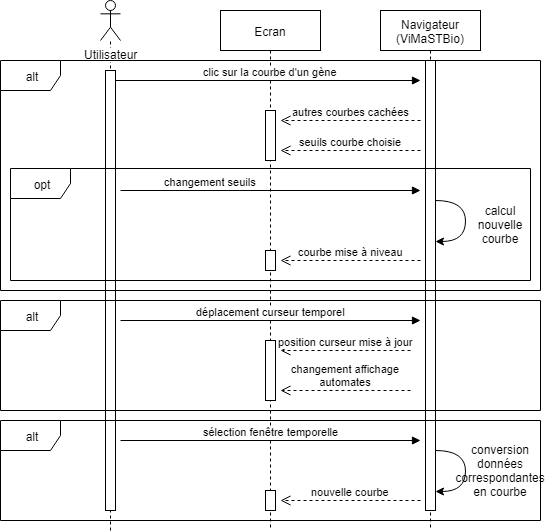
\includegraphics[scale = .6]{images/sequence.png}
   \caption{Diagramme de séquence}
\end{figure}
\bigbreak
\bigbreak
\bigbreak
\bigbreak
\begin{figure}[!h]
    \center
    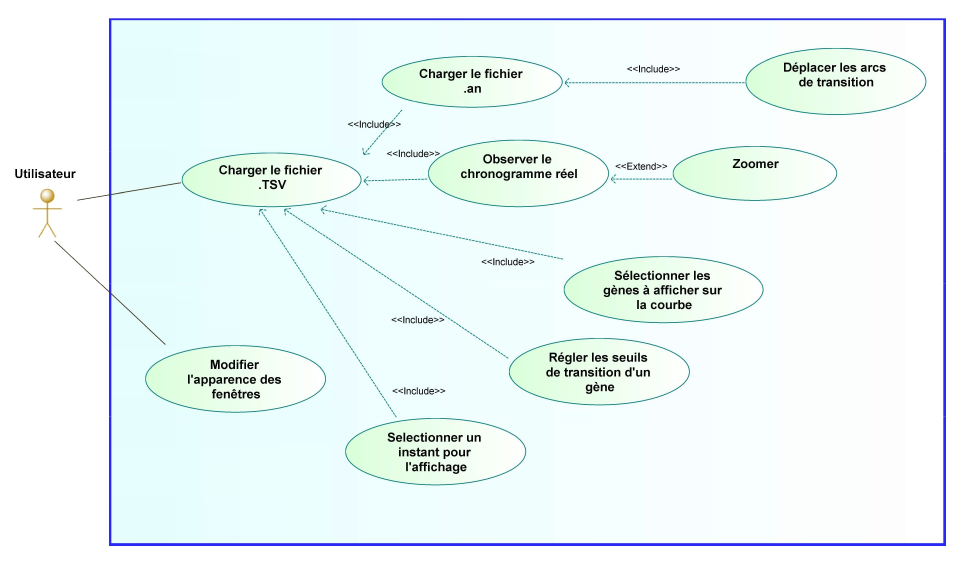
\includegraphics[scale = .45]{images/utilisation.png}
   \caption{Diagramme d'utilisation}
\end{figure}



\clearpage
\newpage

\section{Fonctionnalités de l'outil et réalisation}
\bigbreak


Nous allons dans cette partie présenter les différentes fonctionnalités du logiciel et expliquer comment nous les avons réalisées.

\bigbreak
\subsection{La page html}
\bigbreak

Les fonctionnalités tournant autour de deux axes principaux, le graphe et les automates, il paraissait logique de les afficher dans deux espaces séparés sur la page. Le choix du fenêtrage offre une bonne ergonomie et permet de naviguer dans l’outil de manière confortable (grâce à l’habitude des systèmes d’exploitation). En outre les fonctions créées pour rendre les fenêtres utilisables ont été reprises dans d’autres parties du code (déplacement des flèches de transition des automates, curseurs du RangeSlider).

\begin{figure}[!h]
  \centering
  \includegraphics[scale = .3]{images/html.png}
  \caption{Les deux fenêtres de ViMaSTBio}
\end{figure}
\bigbreak

La structure telle qu’elle apparaît ci-dessus correspond à l’architecture de la page décrite dans le fichier html. Tout le reste est généré par le JavaScript au chargement des fichiers.

Une fois construite, la page html a servi de base à l’intégration des fonctionnalités et a fourni un environnement graphique permettant de tester sans trop de difficultés les nouveautés.

\bigbreak
\newpage
\subsection{Chargement des fichiers .tsv et .an}

\bigbreak

Le programme doit permettre de charger les fichiers .tsv et .an correspondant à des automates et à des chronogrammes. Au lancement du programme deux fenêtres s’affichent. Un bouton dans chacune d’elles permet de charger le fichier correspondant. On ne peut dans chaque fenêtre charger que le bon type de fichier : fichiers .tsv dans la partie graphe et fichiers .an dans la partie automate. Cependant, le choix des fichiers est laissé libre à  l’utilisateur qui peut alors en sélectionner deux qui ne correspondent pas entre eux.  Dans ce cas le logiciel n'affichera que les courbes sans les automates, ou avec les mauvais automates. Il convient donc de faire attention aux fichiers sélectionnés.
\bigbreak

\subsubsection{Lecture et traitement du fichier .tsv}
\bigbreak
La lecture du fichier .tsv se fait avec le programme parseTsv. Le fichier .tsv contient 3 niveaux d’information : le jeu de données, au sein duquel on va retrouver les différentes valeurs pour les gènes ainsi que le temps. On sépare donc les informations au sein d’un tableau qui contient comme première ligne la légende du graphes puis chaque jeu de données contenant les listes des différentes valeurs des gènes à un instant donné.
\bigbreak

\subsubsection{Lecture et traitement du fichier .an}
\bigbreak
La lecture du fichier .an se fait directement dans le fichier readAnFile.js. Il a d'abord fallu réaliser un parser permettant la lecture des fichiers .an fournis par M. Samuel Buchet. Ces derniers contiennent le nom des gènes étudiés, le nombre d'états que chacun d'eux peut prendre ainsi que leurs différentes transitions possibles. En utilisant les expressions régulières nous avons pu extraire ces informations et les stocker dans deux variables globales : auto et transitions. Le premier est un tableau contenant le nombre d’états que peut prendre chacun des gènes. Le second est un dictionnaire contenant pour chacun des gènes, ses transitions et les conditions associées.

Il est important de noter que cette lecture implique que le format des données stockées sur les fichiers .an doivent toujours être le même et suivre une structure identique, ce qui nous avait été confirmé par M. Samuel Buchet. 
\bigbreak

\newpage
\subsection{Représentation des gènes}
\bigbreak
\subsubsection{Représentation graphique et interactions (zoom et légende)}
\bigbreak
L’affichage du graphe se sert pleinement de grafica qui permet d’afficher simplement des graphes. On utilise donc les différentes fonctions dédiées à cela.

Le choix du jeu de données se fait à l’aide de la liste déroulante au-dessus du graphe. Puis, nous n’avons plus qu'à aller chercher les données à afficher.

Nous affichons indépendamment chaque courbes, ce qui permet de les afficher ou non lorsque que l’on clique sur le nom correspondant dans la légende.

Cette légende, dont les données sont récupérées dans le tableau avec toutes les données du graphe, s’affiche grâce à des fonctions standard de graphica. Cependant, c’est sur cet affichage que se superposent les clickListener qui permettent ou non d’afficher les courbes.

Il est aussi possible de zoomer et déplacer le graphe à l’aide de la souris, afin de pouvoir être plus précis dans le choix des seuils. Le zoom et le déplacement se fait grâce à des fonction de grafica qui dissocient les coordonnées dans le graphe et les coordonnées dans la fenêtre. 
\bigbreak
\subsubsection{Représentation des automates}
\bigbreak
Lorsque les gènes sont sélectionnés, il faut pouvoir les représenter sous forme d'automate. Pour ce faire, nous avons choisi, ici aussi, d'utiliser p5 qui offre de nombreuses fonctionnalités de dessin en JavaScript.

Cependant, après avoir longuement cherché s'il permettait de construire automatiquement, ou du moins plus facilement, des automates et n'avoir rien trouvé de concluant, nous avons décidé de les représenter par nous même en dessinant uns à uns les différentes parties avec des arcs, des cercles, des rectangles, etc. Ce fut alors un long travail de tâtonnements et de calculs pour trouver les dimensions adaptées à la représentation voulue, au nombre d'automates à placer dans la page et à leur nombre d'états respectifs.

Ainsi, la représentation des automates se fait en permanence à travers la fonction paintAuto() puisqu’elle utilise la fonction draw de p5, exécutée de manière infinie.
\bigbreak

\subsection{RangeSlider}

À cause du manque de documentation de grafica, il nous paraissait difficile de déplacer efficacement un marqueur dans le graphe à l’aide de la souris : il n’y a pas de relation explicite entre les coordonnées du pointeur de souris et les coordonnées dans le graphe, et une simple règle de proportionnalité ne pouvait pas convenir du fait de la possibilité d’agrandir le graphe ou de déplacer son contenu. Nous avons donc décidé de créer un nouveau composant réalisant l’interface entre l’utilisateur et le graphe.

\begin{figure}[!h]
  \centering
  \includegraphics[scale = .7]{images/slider.png}
  \caption{Un RangeSlider à 5 curseurs}
\end{figure}
N’ayant pas trouvé de librairie supportant plus de deux curseurs à la fois - il en faut n-1 pour chaque automate, avec n le nombre d’états de l’automate - nous avons décidé de coder notre propre classe. Grâce aux possibilités du DOM (html/css/javascript), nous avons pu réaliser sans trop de difficultés un composant hautement personnalisable, intégrant les comportements élémentaires que nous pouvions attendre : non dépassement des curseurs voisins pendant le déplacement, calcul et affichage des mises à jour des valeurs représentées par la position des curseurs.

Cet objet est utilisé pour tracer deux types de marqueur sur le graphe : la barre temporelle et les barres de seuil. que nous allons détailler dans les parties suivantes.
\bigbreak

\subsection{Selection d'une fenêtre temporelle}
\bigbreak
Le chronogramme est déplaçable et il est possible de zoomer afin mieux ajuster les niveaux. Le zoom se fait avec la molette de la souris ou à deux doigts sur un pad. Pour le déplacement de l’affichage, il faut cliquer puis déplacer la fenêtre et relâcher le bouton de la souris.
\bigbreak

\subsection{Selection d'un temps dans le graphe}
\bigbreak
La sélection du temps se fait sensiblement de la même manière que la sélection des seuils. Comme le montre la figure suivante, un curseur indique l’instant actuellement sélectionné pour la représentation des automates :

\vbox{
  \centering
  \includegraphics[scale = 0.5]{images/instant.png}
}
\bigbreak
 On a donc un Slider qui modifie la variable globale time. Cette variable sert à afficher la barre verticale permettant de se repérer dans le graphe.
Cette variable sert aussi à repérer le temps où l’on est, avec ce temps on trouve donc l’abscisse la plus proche dans le tableau array.

Ensuite à l’aide d’une boucle for on regarde pour chaque gène la valeur à cet instant, on la compare ensuite avec les seuils puis on modifie la case correspondante dans la variable globale etatsEnCours. 

\bigbreak

\subsection{Les seuils}
\bigbreak
\subsubsection{Déplacement des seuils de transition}
\bigbreak
L’édition des seuils de transition sur le graphe permet de choisir les valeurs d’activation marquant la frontière entre les états des automates.
Pour accéder au mode d’édition il suffit de cliquer sur les rectangles en couleur sous les gènes :

\begin{figure}[!h]
  \includegraphics[scale = 0.8]{images/couleur_gene.png}
  \caption{Légende représentant des noms de gènes et le rectangle de couleur associée.}
\end{figure}

\begin{figure}[!h]
  \includegraphics[scale = .7]{images/seuil_graphe.png}
  \caption{Mode d’édition du seuil entre les deux états du gène G4.}
\end{figure}

Quand l’édition est lancée, les courbes des autres gènes sont retirées du graphe et l’activation ou la désactivation de l’affichage des courbes (en cliquant sur le nom du gène cette fois) ne sont plus disponibles afin d’éviter que l’application ne fonctionne plus ce qui forcerait à réinitialiser la page. Le curseur déplace la barre à l’abscisse de la valeur affichée au-dessus, et la nouvelle valeur actualise l’état en cours de l’automate sélectionné par l’intermédiaire de la variable globale (on rappelle que les automates sont redessinés en boucle par p5).

Pour quitter le mode d’édition, il suffit de cliquer à nouveau sur la couleur du gène (identique à celle de la barre du RangeSlider) pour ramener à l’affichage normal, ou d’éditer un nouveau gène pour basculer directement sur son mode d’édition.
Attention, si le fichier d’automates correspondant n’est pas chargé, les seuils n’apparaissent pas sur le slide.

\bigbreak
\subsubsection{Les transitions}
\bigbreak

En fonction des seuils établis précédemment, les transitions possibles de chacun des gènes devaient être représentées. Nous avons pour cela dessiné des arcs à l'aide de courbes de Béziers et ajouté à leur côté les conditions nécessaires à leur franchissement lorsqu'il y en a. p5.js proposait alors une solution adaptée avec la fonction Bezier permettant de faire une interpolation à 4 points. 

De plus, les transitions d'un même gène pouvant être nombreuses, il est possible que les différents arcs se chevauchent et que le schéma soit rapidement illisible. Pour éviter cela, nous avons ajouté la possibilité de déplacer les arcs comme nous le souhaitons et ainsi d'agencer l'affichage à notre guide, en plaçant les transitions dans des éléments <div> déplaçables. 



\bigbreak

\subsection{Le lien entre chronogramme et automates}

\bigbreak

Les parties chronogramme réel et automates qui étaient jusqu’ici totalement indépendantes dans leur représentation devaient finalement être liées. En effet, les automates représentent les gènes sélectionnés dans le chronogramme réel et doivent alors, selon l’instant choisi, afficher quel est l’état courant de chacun des gènes. 

Pour ce faire, nous avons principalement utilisé des variables globales actualisées à chaque fois qu’un gène est ajouté ou supprimé ou qu’un instant est sélectionné. La fonction Draw() de p5.js s’exécutant en continu, la représentation se met alors à jour instantanément.

Ceci permet de résoudre une difficulté à laquelle nous avons dû faire face : le chargement des fichiers s’exécute de manière asynchrone(dans les callbacks), c’est-à-dire en parallèle de l’exécution de la suite du code. Ainsi il était difficile de manipuler les valeurs hors des callbacks, sous peine qu’elles ne soient pas encore définies, ce qui devenait contraignant lorsqu’il fallait les partager.

La combinaison des variables globales et des gestionnaires d’événement permet d’outrepasser cette difficulté : l’utilisateur interagit avec la page uniquement quand les composants sont placés, autrement dit après la lecture des fichiers et l’écriture des variables globales.


\newpage

\section{Déroulement du projet}
\bigbreak 
\bigbreak


\subsection{Estimation des coûts}

Nous indiquons ici le temps dédié à chacune des étapes du projet des deux sous-groupes suivi du temps consacré à la mise en commun de ces deux sous-parties.

\subsubsection{Automates}

\begin{flushleft}
\begin{tabular}{|l|c|r|}
  \hline
   Étape & Volume horaire \\
  \hline
  Travail initial sur les fichiers .an & 4h \\
     \hline
  Expressions régulières & 4h \\
  \hline
  Représentations visuelles des automates avec p5.js & ??h\\
  \hline
    Passage aux courbes de Bézier & ??h \\
  \hline
    Déplacement des arcs avec onmouse & ??h\\
  \hline
   Prise en main et calcul des overBox  & 6h \\
  \hline
   Affichage des transitions avec mousePressed() & 8h \\
    \hline
 \end{tabular}
 \end{flushleft}

Au total, nous avons consacré environ \textbf{??} heures pour cette sous-partie. 

\subsubsection{Graphes}

\begin{flushleft}
\begin{tabular}{|l|c|r|}
  \hline
   Étape & Volume horaire \\
  \hline
  Travail initial sur les fichiers .an & 4h \\
     \hline
  Expressions régulières & 4h \\
  \hline
  Représentations visuelles des automates avec p5.js & ??h\\
  \hline
    Passage aux courbes de Bézier & ??h \\
  \hline
    Déplacement des arcs avec onmouse & ??h\\
  \hline
   Prise en main et calcul des overBox  & 6h \\
  \hline
   Affichage des transitions avec mousePressed() & 8h \\
    \hline
 \end{tabular}
 \end{flushleft}

Au total, nous avons consacré environ \textbf{??} heures pour cette sous-partie. 
  
\subsubsection{Mise en commun}

\begin{flushleft}
\begin{tabular}{|l|c|r|}
  \hline
   Étape & Volume horaire \\
  \hline
 Lecture synchrone des fichiers & ??h \\
    \hline
 Rédaction du rapport & ??h \\
 \hline
    
 \end{tabular}
 \end{flushleft}

Au total, nous avons consacré environ \textbf{??} heures pour cette sous-partie.
\bigbreak
Ainsi, ce projet de groupe a été réalisé en \textbf{??} heures de travail. 
  
  
\bigbreak
\bigbreak
\subsection{Difficultés rencontrées}
\bigbreak

\subsubsection{Récupération des données depuis les fichiers .an}
Concernant la partie automates, notre première difficulté fut de récupérer les données des automates à partir des fichiers .an fournis:
\newpage
\begin{figure}
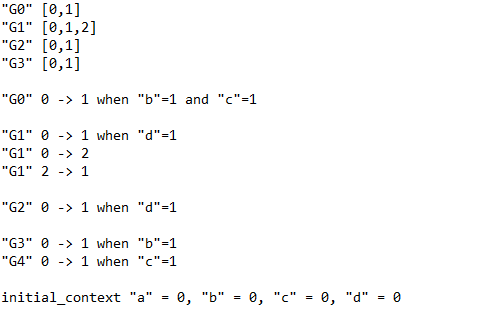
\includegraphics[scale=1]{images/fichier_an.PNG} 
\caption{Exemple de fichier .an}
\end{figure}
Nous avons au départ opté pour la méthode naïve de lire chacune des lignes et d'utiliser la méthode split (selon "when", "and" et "-") mais cette méthode cesse de fonctionner si  il y a plus de 10 automates puisque avoir "G10" au lieu de "G9" décalerait d'une case notre récupération naïve et de même si une transition à deux chiffres prenait place ("b" = 10 au lieu de "b" = 9). 
\newline
Nous avons donc préféré abandonné cette méthode malgré le temps consacré pour utiliser des expressions régulières, méthode bien plus robuste que la précédente.


\subsubsection{Déplacement des courbes}
Toujours dans la partie automates, une autre difficulté rencontrée fut de réussir à pouvoir déplacer les arcs, fonctionnalité nécessaire dès qu'il y a plus de $3$ arcs (représentant les transitions) arrivant ou sortant d'un état puisque la lecture devient alors très pénible:
\newpage
\begin{figure}
  \centering
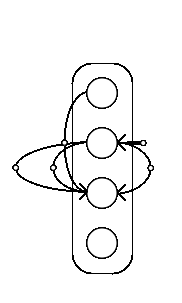
\includegraphics[scale=1]{images/arcs.PNG} 
\caption{Etats surchargés}
\end{figure}
La solution retenue pour rendre ces automates plus lisibles fut de rendre possible le déplacement de ces arcs: l'utilisateur peut ainsi remanier la figure à son goût. Cependant, il fut nécessaire de ré-écrire une portion conséquente du code d'affichage des automates car les méthodes d'affichage initiales écrites en utilisant la fonction \textbf{arc} de p5.js sont incompatibles avec le déplacement conçu par les méthodes \textbf{onmouse}. Ainsi, notre code final utilise les courbes de Bézier pour l'affichage des transitions.


\bigbreak
\subsubsection{Affichage des transitions}
Le dernier obstacle majeur de la partie automates a été celui de l'affichage des transitions puisque l'on voulait initialement que l'affichage des transitions ne s'affichent que lorsque l'utilisateur survole avec sa souris l'état concerné et que ces affichages suivent les arcs déplaçables: 
\begin{figure}
  \centering
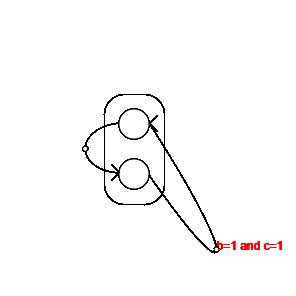
\includegraphics[scale=1]{images/transitions.png} 
\caption{La transition suit l'arc}
\end{figure}
Nous avons du consacré beaucoup de temps pour trouver une solution parmi la documentation souvent très absconse de p5.js et il a fallu ré-écrire cette fonctionnalité à chaque fois que la représentation visuelle des automates et de leurs arcs a été changée. Nous avons finalement retenu le principe de l'overBox: on construit un périmètre autour de l'arc et dès que l'utilisateur passe la souris dans ce périmètre, la transition s'affiche.


\newpage
\section{Axes d'amélioration}
\bigbreak
Les objectifs initialement fixés ont pour une grande majorité été atteints et notre outil est ainsi fonctionnel mais il reste plusieurs améliorations que nous aurions aimé apporter à celle-ci. 

D’abord, nous souhaitions faire une représentation de l'évolution des gènes supposée par les automates sous forme de chronogramme discrétisé. N’ayant pas eu le temps de nous attaquer à cette partie, nous pensons qu’il serait intéressant qu’un futur groupe reprenne le projet afin d’en implémenter cette partie. Cela imposerait de réaliser un programme de décision qui choisirait de franchir les transitions de manière aléatoire dans un premier temps. Un premier chronogramme “prédit” serait alors dessiné. Puis, on peut également imaginer que la possibilité de choisir quelle transition franchir pourrait être donnée à l’utilisateur afin qu’il puisse observer les évolutions qu’il souhaite. Dans le cadre d’une étude biologique, cette fonctionnalité apparaît être intéressante. 

Ensuite, nous avons appris en fin de projet que de nouveaux arcs pourraient être à représenter : ceux dont l’état initial et celui d’arrivée sont le même. Nous n’avons pu modifier le code de telle sorte qu’ils soient affichés joliment et pensons donc qu’il serait possible d’améliorer cette représentation. 

Deux points précis liés aux fenêtres peuvent être corrigés. D’une part, déplacer un élément sélectionne systématiquement une partie du texte présent sur la page à cause du comportement par défaut des navigateurs, mais désactiver ce comportement par défaut empêche d’interagir avec le contenu du graphe (zoom, déplacement) ou avec certains objets html présents dans la page. Nous n’avons pas trouvé comment résoudre ce problème qui ne provoque pas d’erreurs mais peut être légèrement gênant à terme. D’autre part, les fenêtres sont un peu plus dures à redimensionner lorsqu’elles contiennent des barres de défilement puisque la marge de sélection de la bordure est fortement réduite.
Il serait par ailleurs intéressant de rajouter la possibilité de déplacer et de redimensionner le graphe lui-même (comme on peut le faire avec les graphes des tableurs par exemple).

\bigbreak

\newpage
\section{Conclusion}
\bigbreak
\bigbreak

Ce projet a été l'occasion pour nous de consolider nos acquis des cours d'informatique et surtout de toucher à plusieurs domaines inconnus jusque là de la programmation au travers d'un besoin réel. Une grande partie du projet a été consacrée à de la recherche, des tests et de la lecture de documentation afin de comprendre le fonctionnement des différents outils que nous avons manipulés. 

Ainsi, nous avons eu l'occasion d'apprendre comment interagir avec les API (majoritairement celles de Google) pour les logiciels les fournissant et de trouver une alternative pour les autres, via l'envoi de requêtes POST pour le site Doodle en l'occurrence. 

D'autre part, nous avons appris à concevoir une application Web dans son ensemble via le framework Flask. Pour le déploiement, nous avons suivi plusieurs pistes sans succès, notamment via Firebase, mais nous nous sommes finalement accordés sur le choix de Heroku, service le plus adapté aux applications Flask. 

Enfin, les différents problèmes rencontrés au cours du projet nous ont permis d'apprendre à trouver des alternatives notamment lorsque la solution n'était pas immédiate. Par exemple, le problème de l'authentification d'un compte Google nous a valu plusieurs heures de recherches et de tests avant de trouver une solution. 

Ce projet est donc un projet polyvalent qui nous a permis de developper des connaissances dans de nombreux domaines. 

\newpage
\nocite{*}
\bibliographystyle{plain}
\bibliography{fichiers/bibliographie}

\end{document}
